\documentclass[aspectratio=169,professionalfonts]{beamer}

\usepackage{booktabs}
\usepackage{tabularx}
\usepackage{array}
\usepackage{graphicx}
\usepackage{xcolor}
\usepackage{tikz}
\usepackage{ragged2e}
\usepackage{amsmath}
\usepackage{amssymb}
\usepackage{hyperref}
\usetikzlibrary{positioning,arrows.meta,fit,calc,shapes.geometric}

\usetheme{Madrid}
\setbeamertemplate{blocks}[rounded][shadow=false]
\setbeamertemplate{navigation symbols}{}
\setbeamertemplate{caption}[numbered]

\definecolor{ProjBlue}{RGB}{28,67,133}
\definecolor{ProjOrange}{RGB}{210,102,28}
\definecolor{ProjGreen}{RGB}{52,132,67}
\definecolor{ProjGray}{RGB}{70,70,70}

\setbeamercolor{structure}{fg=ProjBlue}
\setbeamercolor{title}{fg=ProjBlue}
\setbeamercolor{frametitle}{bg=ProjBlue!7, fg=black}
\setbeamercolor{author}{fg=ProjGray}
\setbeamercolor{institute}{fg=ProjGray}
\setbeamercolor{alerted text}{fg=ProjOrange}
\setbeamercolor{block title}{bg=ProjBlue!10, fg=black}
\setbeamercolor{block body}{bg=black!2, fg=black}
\setbeamerfont{frametitle}{series=\bfseries}

\newcolumntype{Y}{>{\RaggedRight\arraybackslash}X}
\newcommand{\good}{\textcolor{ProjGreen}{\checkmark}}
\newcommand{\fig}[1]{\includegraphics[width=\linewidth]{#1}}
\newcommand{\smfig}[2][]{\includegraphics[#1]{#2}}

\title[OVD and Visual Grounding]{Open-Vocabulary Object Detection and Visual Grounding}
\subtitle{Full-split reproduction, evaluation, and analysis}
\author{Zheng Renjie \quad Lin Hongyu \quad He Jiayang \quad Deng Haotian}
\institute{Southern University of Science and Technology}
\date{CS308 Final Project Defense \quad June 2026}

\begin{document}

\begin{frame}[plain]
  \vspace*{0.8cm}
  \begin{center}
    {\usebeamerfont{title}\color{ProjBlue}\bfseries\fontsize{26}{30}\selectfont
    Open-Vocabulary Object Detection\\[0.15em]
    and Visual Grounding}

    \vspace{0.55cm}
    {\large Full-split reproduction, evaluation, and analysis}

    \vspace{0.8cm}
    \begin{beamercolorbox}[wd=0.82\textwidth,sep=0.8em,rounded=true,center]{block body}
      \normalsize
      Zheng Renjie \quad Lin Hongyu \quad He Jiayang \quad Deng Haotian

      \vspace{0.25em}
      \footnotesize
      Southern University of Science and Technology

      \vspace{0.25em}
      \small
      CS308 Final Project Defense \quad June 2026
    \end{beamercolorbox}

    \vspace{0.55cm}
    \begin{tabular}{@{}ccc@{}}
      \textcolor{ProjBlue}{\rule{1.8cm}{0.16cm}} &
      \textcolor{ProjOrange}{\rule{1.8cm}{0.16cm}} &
      \textcolor{ProjGreen}{\rule{1.8cm}{0.16cm}} \\
    \end{tabular}

    \vfill
    \footnotesize
    Reproducible benchmark comparison on COCO and RefCOCO
  \end{center}
\end{frame}

\begin{frame}{Roadmap}
  \begin{columns}[T,onlytextwidth]
    \column{0.48\textwidth}
    \begin{block}{Main story}
      \begin{enumerate}
        \item Motivation and task scope
        \item Related work and model choice
        \item Approach and evaluation pipeline
        \item Full COCO and RefCOCO results
        \item Ablations, qualitative analysis, and takeaways
      \end{enumerate}
    \end{block}

    \column{0.48\textwidth}
    \begin{block}{What to remember}
      \begin{itemize}
        \item Full-split results are the only headline numbers.
        \item RefCOCO uses all expressions, not just a diagnostic slice.
        \item The comparison covers accuracy, speed, memory, and robustness.
      \end{itemize}
    \end{block}
  \end{columns}
\end{frame}

\section{Motivation}

\begin{frame}{What Problem Are We Solving?}
  \begin{columns}[T,onlytextwidth]
    \column{0.56\textwidth}
    \begin{block}{Task}
      Open-vocabulary detection asks a detector to localize arbitrary text prompts.
      Visual grounding goes one step further and asks for the exact instance
      described by a referring expression.
    \end{block}

    \begin{itemize}
      \item Fixed-label detectors cannot directly handle new words without retraining.
      \item Grounding is harder than category detection because the model must resolve
            attributes, relations, and instance ambiguity.
      \item Our goal is not to train a new model, but to reproduce and compare strong
            pretrained baselines under one rigorous protocol.
    \end{itemize}

    \column{0.40\textwidth}
    \begin{block}{Project Goal}
      \centering
      \large
      Reproduce \\
      Evaluate \\
      Analyze \\
      Explain
    \end{block}

    \vspace{0.35em}
    \footnotesize
    The final report and code answer both sides of the assignment:
    open-vocabulary detection and visual grounding.
  \end{columns}
\end{frame}

\begin{frame}{Related Work and Model Choice}
  \begin{columns}[T,onlytextwidth]
    \column{0.32\textwidth}
    \begin{block}{OWL-ViT}
      \small
      A compact text-image similarity detector. It is the lightest baseline in our comparison, but not the strongest on accuracy.
    \end{block}

    \column{0.32\textwidth}
    \begin{block}{Grounding DINO}
      \small
      A grounding-oriented detector. It gives the best accuracy on both COCO and RefCOCO, so it serves as the accuracy-first reference.
    \end{block}

    \column{0.32\textwidth}
    \begin{block}{YOLO-World}
      \small
      A real-time open-vocabulary detector. It is the best deployment-oriented baseline because it balances speed and recall well.
    \end{block}
  \end{columns}

  \vspace{0.35em}
  \begin{alertblock}{Why these three?}
    They span the accuracy-speed-memory spectrum, which matches the application-oriented scope of the project.
  \end{alertblock}
\end{frame}

\begin{frame}{What We Built}
  \small
  \begin{tabularx}{\textwidth}{>{\bfseries}p{3.35cm}Y}
    Task coverage & Both open-vocabulary object detection and visual grounding are evaluated. \\
    Model coverage & OWL-ViT, Grounding DINO, and YOLO-World are all reproduced with pretrained weights. \\
    Data coverage & Full COCO val2017 and full RefCOCO val with all expressions are used for the final claims. \\
    Metric coverage & AP / AP50 / AP75 / AR100, grounding Acc@0.5 / Acc@0.75 / mean IoU, FPS, and peak VRAM. \\
    Extra analysis & Score-threshold sensitivity, OWL-ViT NMS, and qualitative examples are included. \\
    Reproducibility & Shared config block, manifest caching, local RefCOCO parquet fallback, and timestamped server logs. \\
  \end{tabularx}

  \vspace{0.5em}
  \begin{alertblock}{Important}
    The 100-row and 500-image results are diagnostics only. All headline claims in the report come from full-split runs.
  \end{alertblock}
\end{frame}

\section{Approach}

\begin{frame}{Implementation Map}
  \begin{columns}[T,onlytextwidth]
    \column{0.49\textwidth}
    \begin{block}{Model wrappers}
      \small
      \begin{itemize}
        \item \texttt{evaluate\_coco\_*.py}: full COCO val2017 inference, predictions, timing, and VRAM.
        \item \texttt{evaluate\_refcoco.py}: full RefCOCO val, all expressions, local parquet fallback.
        \item \texttt{evaluate\_threshold\_sensitivity.py}: re-scores saved COCO predictions under multiple thresholds.
      \end{itemize}
    \end{block}

    \column{0.49\textwidth}
    \begin{block}{Shared infrastructure}
      \small
      \begin{itemize}
        \item One output schema: image id, prompt id, score, box, runtime, and peak memory.
        \item \texttt{coco\_eval\_utils.py} and \texttt{generate\_report\_figures.py} keep metrics and plots consistent.
        \item \texttt{run\_full\_suite\_4gpu\_server.sh} orchestrates the 4-GPU rerun with timestamped logs.
      \end{itemize}
    \end{block}
  \end{columns}

  \vspace{0.35em}
  \begin{alertblock}{Normalization idea}
    Converting all model APIs to one schema is what makes the comparison fair: same data, same metrics, same reporting path.
  \end{alertblock}
\end{frame}

\begin{frame}{Unified Pipeline}
  \centering
  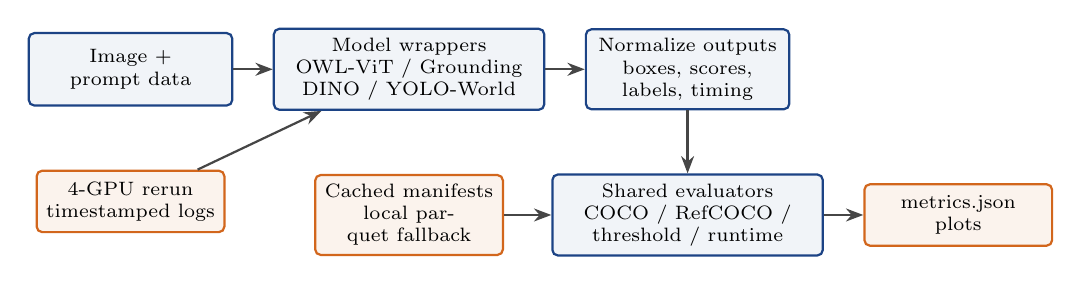
\begin{tikzpicture}[
      node distance=5mm and 5mm,
      font=\scriptsize,
      block/.style={draw=ProjBlue, thick, rounded corners=2pt, fill=ProjBlue!6,
                    text width=2.35cm, minimum height=0.92cm, align=center},
      wideblock/.style={draw=ProjBlue, thick, rounded corners=2pt, fill=ProjBlue!6,
                    text width=3.2cm, minimum height=0.92cm, align=center},
      smallblock/.style={draw=ProjOrange, thick, rounded corners=2pt, fill=ProjOrange!8,
                         text width=2.15cm, minimum height=0.78cm, align=center},
      arrow/.style={-{Stealth[length=2.2mm]}, thick, draw=ProjGray}
    ]
    \node[block] (input) {Image + prompt data};
    \node[wideblock, right=of input] (model) {Model wrappers\\OWL-ViT / Grounding DINO / YOLO-World};
    \node[block, right=of model] (norm) {Normalize outputs\\boxes, scores, labels, timing};

    \node[smallblock, below=8mm of input] (server) {4-GPU rerun\\timestamped logs};
    \node[smallblock, below=8mm of model] (cache) {Cached manifests\\local parquet fallback};
    \node[wideblock, below=8mm of norm] (eval) {Shared evaluators\\COCO / RefCOCO / threshold / runtime};
    \node[smallblock, right=of eval] (out) {metrics.json\\plots};

    \draw[arrow] (input) -- (model);
    \draw[arrow] (model) -- (norm);
    \draw[arrow] (norm) -- (eval);
    \draw[arrow] (eval) -- (out);
    \draw[arrow] (cache) -- (eval);
    \draw[arrow] (server) -- (model);
  \end{tikzpicture}

  \vspace{0.45em}
  \begin{itemize}
    \item Same code path for accuracy, speed, and qualitative visualization.
    \item Same output directory layout for every full-split rerun.
    \item Cached manifests prevent silent changes in the benchmark data.
  \end{itemize}
\end{frame}

\begin{frame}{Experimental Setup}
  \begin{columns}[T,onlytextwidth]
    \column{0.48\textwidth}
    \begin{block}{Hardware and software}
      \footnotesize
      \begin{itemize}
        \item 4 x TITAN RTX server
        \item NVIDIA driver 550.120, CUDA 12.4
        \item PyTorch 2.6.0+cu124, Torchvision 0.21.0+cu124
        \item Transformers 5.5.3, Ultralytics 8.4.70
      \end{itemize}
    \end{block}

    \column{0.48\textwidth}
    \begin{block}{Metrics}
      \footnotesize
      \begin{itemize}
        \item COCO: AP, AP50, AP75, scale AP, AR100
        \item RefCOCO: Acc@0.5, Acc@0.75, mean IoU
        \item Efficiency: pipeline FPS and peak allocated GPU memory
        \item Ablations: threshold sensitivity and NMS
      \end{itemize}
    \end{block}
  \end{columns}

  \vspace{0.35em}
  \begin{columns}[T,onlytextwidth]
    \column{0.48\textwidth}
    \begin{block}{Formal evaluation}
      \footnotesize
      \begin{itemize}
        \item COCO val2017: 5,000 images, 80 category prompts
        \item RefCOCO val: 8,811 rows, 25,080 expressions
        \item Diagnostics only: 100-row / 500-image subsets
      \end{itemize}
    \end{block}

    \column{0.48\textwidth}
    \begin{alertblock}{What this means}
      \footnotesize
      The slides and report use only full-split numbers for the final claims.
      Smaller runs are retained for debugging and sanity checks.
    \end{alertblock}
  \end{columns}
\end{frame}

\section{Results}

\begin{frame}{COCO Detection Results}
  \begin{columns}[T,onlytextwidth]
    \column{0.60\textwidth}
    \fig{../report/figures/coco_metrics.png}

    \column{0.38\textwidth}
    \begin{block}{Key numbers}
      \small
      \begin{itemize}
        \item Grounding DINO: AP 0.421, best across all AP variants.
        \item YOLO-World: AP 0.366, best AR100 0.547.
        \item OWL-ViT: AP 0.237, compact baseline but weakest accuracy.
      \end{itemize}
    \end{block}

    \begin{block}{Interpretation}
      \small
      Grounding DINO is the strongest accuracy-first choice.
      YOLO-World is the best recall-efficiency compromise.
    \end{block}
  \end{columns}
\end{frame}

\begin{frame}{Efficiency and Deployment Trade-off}
  \begin{columns}[T,onlytextwidth]
    \column{0.62\textwidth}
    \fig{../report/figures/efficiency.png}

    \column{0.36\textwidth}
    \begin{block}{Pipeline timing}
      \small
      \begin{itemize}
        \item OWL-ViT: 24.3 FPS, 350 MB
        \item Grounding DINO: 4.5 FPS, 2357 MB
        \item YOLO-World: 84.6 FPS, 715 MB
      \end{itemize}
    \end{block}

    \begin{alertblock}{Takeaway}
      Higher accuracy does not mean higher throughput.
      The right model depends on the deployment budget.
    \end{alertblock}
  \end{columns}
\end{frame}

\begin{frame}{RefCOCO Grounding Results}
  \begin{columns}[T,onlytextwidth]
    \column{0.60\textwidth}
    \fig{../report/figures/refcoco_grounding.png}

    \column{0.38\textwidth}
    \begin{block}{Why this is stricter}
      \small
      RefCOCO evaluates the exact referred instance, not just the category name.
      The final run uses every expression, so it is much harder than a 100-row diagnostic.
    \end{block}

    \begin{block}{Numbers}
      \small
      \begin{itemize}
        \item Grounding DINO: 51.1\% / 45.6\% / 0.514
        \item OWL-ViT: 42.5\% / 34.2\% / 0.423
        \item YOLO-World: 41.4\% / 36.2\% / 0.422
      \end{itemize}
    \end{block}
  \end{columns}
\end{frame}

\begin{frame}{Threshold Sensitivity and NMS}
  \begin{columns}[T,onlytextwidth]
    \column{0.64\textwidth}
    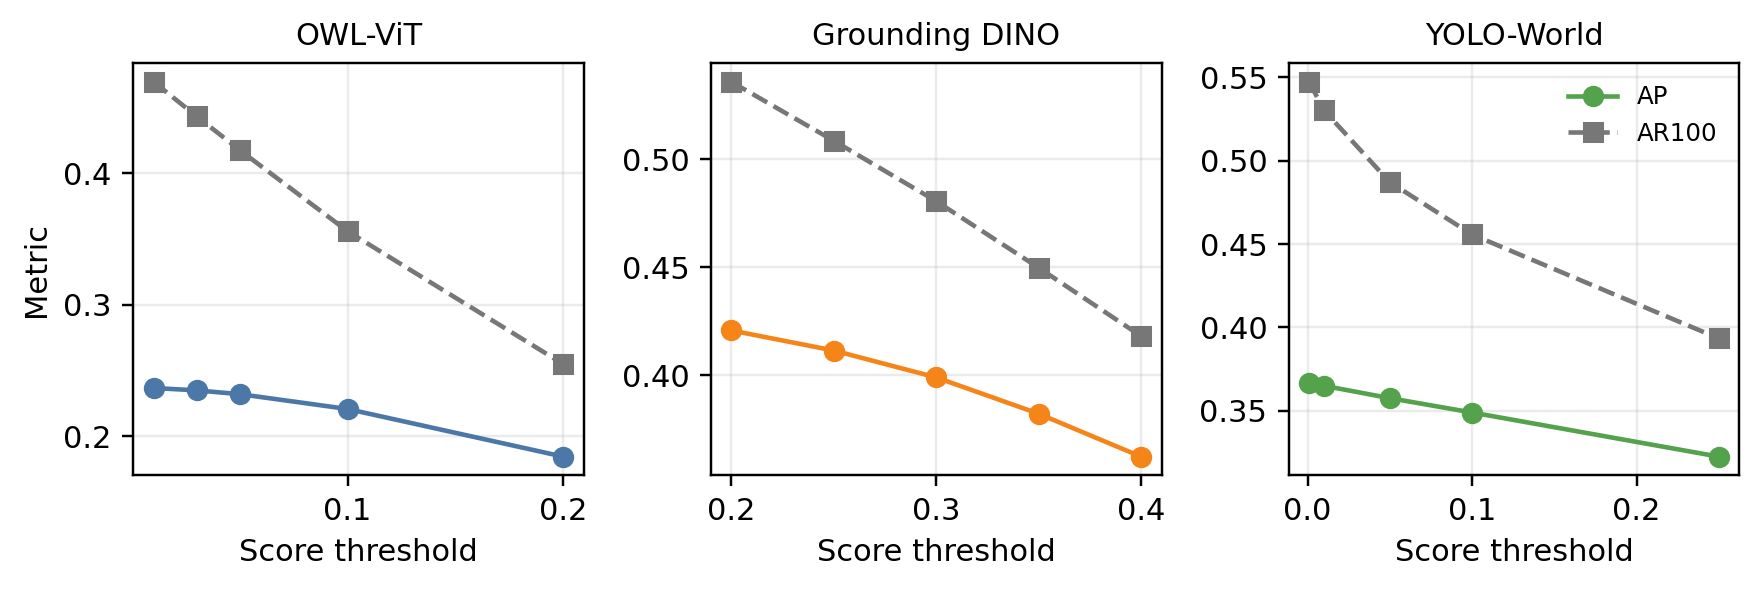
\includegraphics[width=\linewidth,height=0.49\textheight,keepaspectratio]{../report/figures/threshold_sensitivity.png}

    \column{0.34\textwidth}
    \footnotesize
    \begin{block}{Main observation}
      Thresholds are model-specific. Cleaner visualizations usually mean lower recall, not better AP.
    \end{block}

    \begin{block}{Metric trend}
      \begin{itemize}
        \item OWL-ViT AP: 0.237 \textrightarrow{} 0.184.
        \item Grounding DINO AP: 0.421 \textrightarrow{} 0.362.
        \item YOLO-World AP: 0.366 \textrightarrow{} 0.322.
      \end{itemize}
    \end{block}

  \end{columns}
\end{frame}

\begin{frame}{Qualitative Examples and Failure Modes}
  \begin{columns}[T,onlytextwidth]
    \column{0.74\textwidth}
    \centering
    {\setlength{\tabcolsep}{2pt}
    \begin{tabular}{@{}cc@{}}
      \smfig[width=0.66\linewidth,height=0.27\textheight,keepaspectratio]{../report/figures/owlvit_workspace.jpg} &
      \smfig[width=0.66\linewidth,height=0.27\textheight,keepaspectratio]{../report/figures/grounding_dino_workspace.jpg} \\
      {\scriptsize OWL-ViT workspace} & {\scriptsize Grounding DINO workspace} \\
      \smfig[width=0.66\linewidth,height=0.27\textheight,keepaspectratio]{../report/figures/owlvit_traffic.jpg} &
      \smfig[width=0.66\linewidth,height=0.27\textheight,keepaspectratio]{../report/figures/grounding_dino_traffic.jpg} \\
      {\scriptsize OWL-ViT traffic} & {\scriptsize Grounding DINO traffic}
    \end{tabular}}

    \column{0.24\textwidth}
    \begin{block}{Two comparisons}
      \scriptsize
      \begin{itemize}
        \item Workspace: both models detect the main objects.
        \item Traffic: small or occluded objects are harder.
        \item Grounding DINO is usually tighter.
      \end{itemize}
    \end{block}

    \begin{block}{Common errors}
      \scriptsize
      \begin{itemize}
        \item duplicate boxes
        \item nearby-object confusion
        \item spatial relation failures
      \end{itemize}
    \end{block}
  \end{columns}
\end{frame}

\section{Summary}

\begin{frame}{Limitations and Takeaways}
  \begin{columns}[T,onlytextwidth]
    \column{0.49\textwidth}
    \begin{block}{Limitations}
      \small
      \begin{itemize}
        \item No fine-tuning or learned calibration.
        \item COCO and RefCOCO are still curated benchmarks, not open-world data.
        \item Runtime depends on hardware, precision, and input resolution.
      \end{itemize}
    \end{block}

    \begin{block}{Future work}
      \small
      \begin{itemize}
        \item LVIS or ODinW for longer-tail categories
        \item Flickr30K Entities for caption-style grounding
        \item Prompt paraphrase study for robustness
      \end{itemize}
    \end{block}

    \column{0.49\textwidth}
    \begin{block}{Final takeaways}
      \small
      \begin{itemize}
        \item Grounding DINO: best accuracy on both COCO and RefCOCO.
        \item YOLO-World: best speed / efficiency trade-off.
        \item OWL-ViT: simplest baseline and low-memory reference.
        \item The project is fully reproducible and based on full-split results.
      \end{itemize}
    \end{block}

    \begin{alertblock}{One-sentence defense}
      \footnotesize
      We did not just run a demo. We built a unified, reproducible benchmark for open-vocabulary detection and grounding.
    \end{alertblock}
  \end{columns}
\end{frame}

\begin{frame}
  \centering
  \vspace{1.2em}
  \Huge Thank you

  \vspace{0.7em}
  \large Questions are welcome.
\end{frame}

\appendix

\begin{frame}{Backup: Exact Full-Split Numbers}
  \scriptsize
  \begin{columns}[T,onlytextwidth]
    \column{0.49\textwidth}
    \begin{block}{COCO val2017}
      \resizebox{\linewidth}{!}{%
      \begin{tabular}{lrrrrr}
        \toprule
        Model & AP & AP50 & AP75 & AR100 & FPS \\
        \midrule
        OWL-ViT & 0.237 & 0.385 & 0.249 & 0.469 & 24.3 \\
        Grounding DINO & \textbf{0.421} & \textbf{0.557} & \textbf{0.457} & 0.536 & 4.5 \\
        YOLO-World & 0.366 & 0.510 & 0.398 & \textbf{0.547} & \textbf{84.6} \\
        \bottomrule
      \end{tabular}}
    \end{block}

    \column{0.49\textwidth}
    \begin{block}{RefCOCO val}
      \resizebox{\linewidth}{!}{%
      \begin{tabular}{lrrrr}
        \toprule
        Model & Acc@0.5 & Acc@0.75 & Mean IoU & FPS \\
        \midrule
        OWL-ViT & 0.425 & 0.342 & 0.423 & 29.9 \\
        Grounding DINO & \textbf{0.511} & \textbf{0.456} & \textbf{0.514} & 3.1 \\
        YOLO-World & 0.414 & 0.362 & 0.422 & \textbf{115.1} \\
        \bottomrule
      \end{tabular}}
    \end{block}

    \begin{block}{Diagnostic NMS check}
      \small
      OWL-ViT 100-image subset: AP 0.336 \textrightarrow{} 0.323 and AR100 0.520 \textrightarrow{} 0.475 after class-wise NMS.
    \end{block}
  \end{columns}
\end{frame}

\begin{frame}{Backup: Reproducibility Checklist}
  \small
  \begin{itemize}
    \item Server rerun script: \texttt{bash scripts/run\_full\_suite\_4gpu\_server.sh}
    \item Shared configuration block: \texttt{COCO\_MAX\_IMAGES=0}, \texttt{REFCOCO\_MAX\_ROWS=0}, \texttt{REFCOCO\_EXPRESSION\_MODE=all}
    \item RefCOCO manifest fallback: local Hugging Face parquet snapshot under \texttt{data/refcoco/hf\_snapshot}
    \item Final artifact directories: \texttt{outputs/server\_2026\_06/} and \texttt{logs/server\_2026\_06/}
    \item Paper format: IEEE conference style, fully compiled locally before submission
  \end{itemize}
\end{frame}

\end{document}
